\begin{center}
\fbox{\fbox{\parbox{6.5in}{\centering
\begin{flushleft}

\vspace{2mm}
\hspace{5mm}
\textbf{\underline{Ruutfunktsioon $y=ax^{2}+bx+c$ ja selle graafik}}

\vspace{2mm}
\hspace{5mm}
Ruutfunktsioon koosneb \textbf{ruutliikmest} $ax^{2}$ (kusjuures $a \neq 0 $, muidu ei oleks ruutfunktsioon),\\ \hspace{5mm} \textbf{lineaarliikmest} $bx$ ning \textbf{vabaliikmest} $c$.

\vspace{2mm}
\hspace{5mm}
Ruutfunktsiooni graafikuks on parabool, mis näeb välja nõnda:

\begin{center}
\begin{minipage}{7cm}
  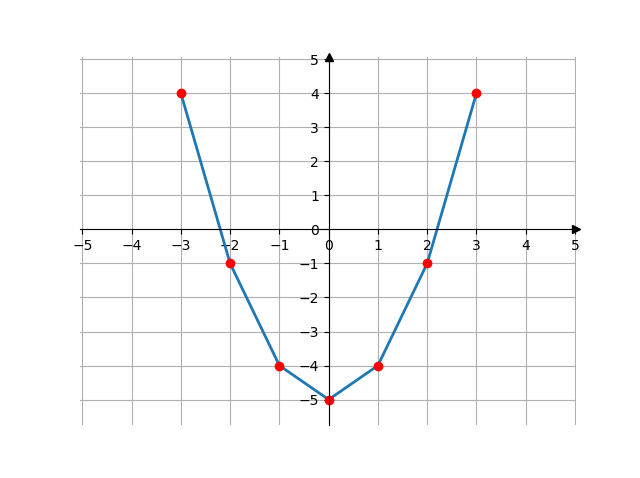
\includegraphics[width=7cm]{36_joonis1.png}
  \captionof{figure}{$y=x^{2}-5$}
  \label{36_joonis1}
\end{minipage}
\hspace{.05\linewidth}
\begin{minipage}{.45\linewidth}
  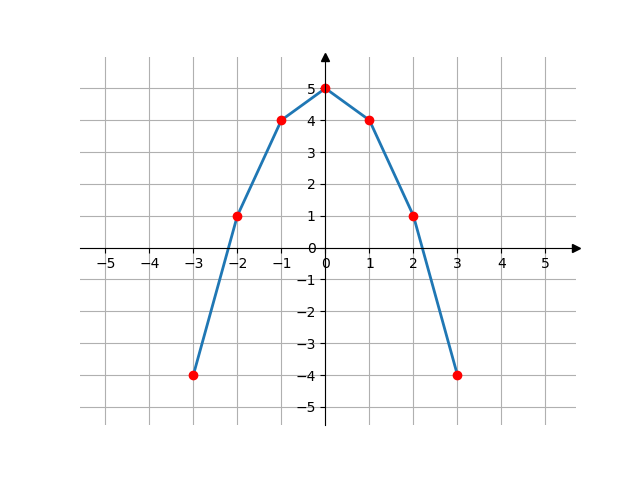
\includegraphics[width=7cm]{36_joonis2.png}
  \captionof{figure}{$y=-x^{2}+5$}
  \label{36_joonis1}
\end{minipage}
\end{center}


\vspace{2mm}
\hspace{5mm}
Nagu näha, näeb parabool kausi moodi välja. 


\begin{itemize}
\item Kui $a$ on positiivne ($a>0$), siis on kauss avatud ülespoole (joonis \ref{36_joonis1}).
\item Kui $a$ on negatiivne ($a<0$), siis on kauss avatud allapoole (joonis \ref{36_joonis2}). 
\end{itemize}

\vspace{2mm}
\hspace{5mm}
Mõned tähelepanekud kordajate $a$, $b$ ja $c$ osas veel:

\begin{itemize}
\item Mida suurem kordaja $\mathbf{a}$, seda kitsam meie parabool/kauss on.
\item Kordajad $\mathbf{b}$ ja $\mathbf{c}$ parabooli kuju ei mõjuta. Need kordajad määravad vaid parabooli asukoha graafikul.
\item Kordaja $\mathbf{c}$ nihutab kõverat positiivse väärtuse korral ülespoole ning negatiivse väärtuse korral allapoole.
\end{itemize} 

\vspace{2mm}
\hspace{5mm}
Parabooli tippu, ehk $+a$ korral madalamat punkti ning $-a$ korral kõrgeimat punkti, nimetatakse\\ \hspace{5mm} \textbf{haripunktiks}. Parabooli punkte, mis puutuvad kokku $x$ - teljega (ehk kus $y=0$) nimetatakse\\ \hspace{5mm} \textbf{nullkohtadeks}. 

\vspace{5mm}
\hspace{5mm}
\textbf{\underline{Ruutfunktsiooni graafiku joonestamine}}

\vspace{2mm}
\hspace{5mm}
Ruutfunktsiooni graafiku joonestamisel tohib lähtuda peatükkist \ref{peatükk_8}. Kuna ruutfunktsioon ei ole meil\\ \hspace{5mm} sirge, siis tuleb meil võtta rohkem kui kaks punkti. 

\vspace{2mm}
\hspace{5mm}
\textbf{Näiteks:} Leiame funktsiooni $y=x^{2}-5$ graafiku.

\vspace{2mm}
\hspace{5mm}
Valime $x$ - ideks järgmised väärtused: $x=\{-3, -2, -1, 0, 1, 2, 3 \}$. 


\end{flushleft}
}}}
\end{center}

\pagebreak


\begin{center}
\fbox{\fbox{\parbox{6.5in}{\centering
\begin{flushleft}

\vspace{5mm}
\hspace{5mm}
Koostame väärtustetabeli nagu peatükkis \ref{peatükk_8}:
\hspace{5mm}
\begin{tabular}{|c|c|c|c|c|c|c|c}
x & -3 & -2 & -1 & 0 & 1 & 2 & 3\\
\hline 
y & 4 & -1 & -4 & -5 & -4 & -1 & 4
\end{tabular}


\vspace{2mm}
\hspace{5mm}
Kanname punktid graafikule ja ühendame punktid vasakult paremale liikudes (joonis \ref{36_joonis1}).

\vspace{5mm}
\hspace{5mm}
\textbf{\underline{Punkti asumine joonel}}

\vspace{2mm}
\hspace{5mm}
Selleks, et veenduda, kas punkt asub joonel või mitte, tuleb asetada punkti koordinaadid vastavasse\\ \hspace{5mm} funktsiooni valemisse ning kontrollida kas võrdus kehtib (ehk kas VP=PP). Punkti koordinaadid olid\\ \hspace{5mm} kirjas nõnda: (x,y).

\vspace{2mm}
\hspace{5mm}
\textbf{Näiteks:}

\vspace{2mm}
\hspace{5mm}
Kontrollime, kas punkt A(2,-3) ja punkt B(-4, 11) asuvad joonel, mis on määratud funktsiooniga\\ \hspace{5mm} $y=x^{2}-5$.

\vspace{2mm}
\hspace{5mm}
Alustame punktist A. Asetame punktile A vastavad koordinaadid funktsiooni valemisse:

\[ y=x^{2}-5 \hspace{3mm} \longrightarrow \hspace{3mm} \left[ \begin{tabular}{c}
Asendame $A(2, -3)$\\
ehk $x=2$ ja $y=-3$
\end{tabular} \right] \hspace{3mm} \longrightarrow  \]

\[ \longrightarrow \hspace{3mm} -3 = 2^{2}-5 \hspace{3mm} \longrightarrow \hspace{3mm} -3 = 4 -5 \hspace{3mm} \longrightarrow \hspace{3mm} -3 \neq -1 \]

\hspace{5mm}
kuna võrdus ei kehti, siis järelikult punkt A \textbf{ei kuulu} funktsiooni joonele.

\vspace{2mm}
\hspace{5mm}
Kontrollime punkti B.

\[ y=x^{2}-5 \hspace{3mm} \longrightarrow \hspace{3mm} \left[ \begin{tabular}{c}
Asendame $B(-4, 11)$\\
ehk $x=-4$ ja $y=11$
\end{tabular} \right] \hspace{3mm} \longrightarrow  \]

\[ \longrightarrow \hspace{3mm} 11 = (-4)^{2}-5 \hspace{3mm} \longrightarrow \hspace{3mm} 11 = 16 -5 \hspace{3mm} \longrightarrow \hspace{3mm} 11 = 11 \]

\hspace{5mm}
kuna võrdus kehtib, siis järelikult punkt B \textbf{kuulub} funktsiooni joonele.
\end{flushleft}
}}}
\end{center}



\vspace{0.5cm}

\textbf{Märkmed}\\
\vspace{2mm}
\begin{mdframed}[style=graphpaper]
\vspace{6cm}
\end{mdframed}
